% Python-generated figure includes (matplotlib output under assets/).

\graphicspath{{../assets/}}

\section{Automation Impact Graph}
\label{sec:python-graph}

The graph below illustrates workflow maturity, automation impact, and human supervision
requirements across task categories \cite{arxiv2506workagents}.

\begin{figure}[htbp]
  \centering
  \IfFileExists{../assets/automation_impact_graph.png}{%
    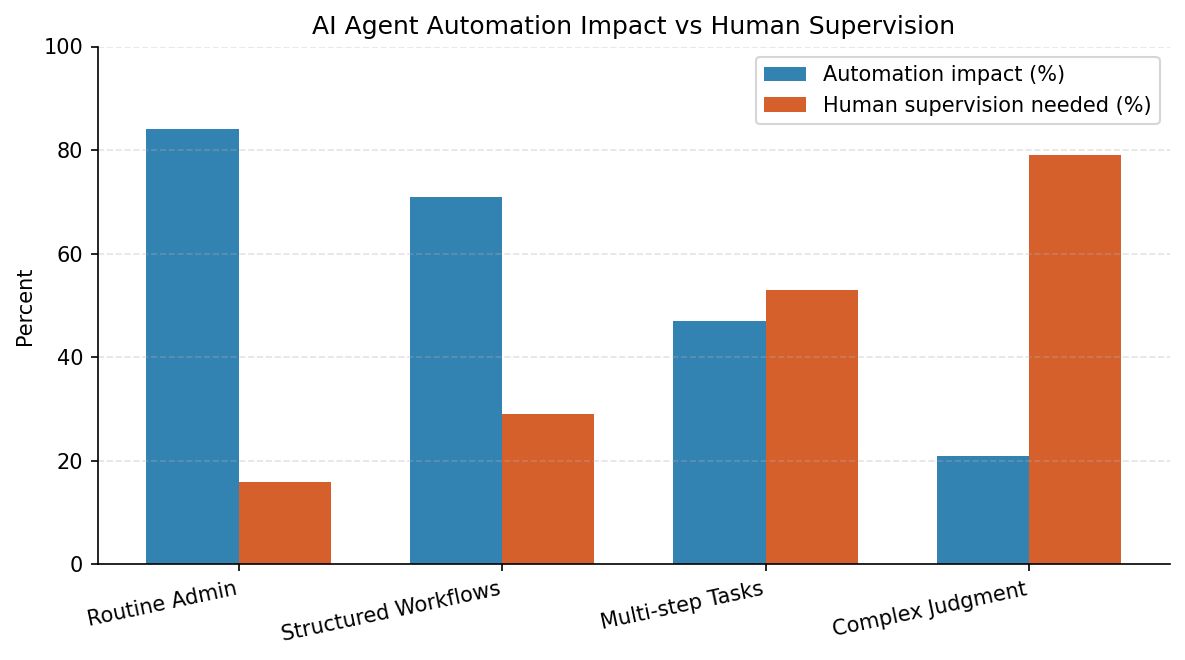
\includegraphics[width=0.92\linewidth]{automation_impact_graph.png}%
  }{%
    \begin{warningbox}{Figure unavailable}
      The automation impact chart is not available in the build output.
    \end{warningbox}
  }
  \caption{Python-generated graph: automation impact vs human supervision by task type.}
  \label{fig:automation-impact-graph}
\end{figure}

Routine administrative work shows the highest automation impact in this model, while complex
judgment tasks retain the highest supervision requirement \cite{recomaijobroles}. That
pattern supports a tiered adoption strategy: automate structured spines first, keep humans
on exception handling and approval gates \cite{arxiv2506workagents}.

\begin{insightbox}{Graph vs diagram}
The workflow diagram in Chapter~2 explains \textbf{how} real work moves through agentic
automation. This chart estimates \textbf{where} automation pressure and human supervision
concentrate in practice.
\end{insightbox}
